
%(BEGIN_QUESTION)
% Copyright 2012, Tony R. Kuphaldt, released under the Creative Commons Attribution License (v 1.0)
% This means you may do almost anything with this work of mine, so long as you give me proper credit

The radius of a {\it Fresnel zone} between two radio antennas may be predicted by the following equation:

$$r = \sqrt{{n \lambda d_1 d_2} \over D}$$

$$\includegraphics[width=15.5cm]{i01339x01.eps}$$

Manipulate this equation to solve for each of the following variables:

\vskip 10pt

$d_1 =$

\vskip 10pt

$D =$

\vskip 10pt

$\lambda =$

\vskip 10pt

\underbar{file i01339}
%(END_QUESTION)





%(BEGIN_ANSWER)

$$d_1 = {D r^2 \over n \lambda d_2}$$

\vskip 20pt

$$D = {n \lambda d_1 d_2 \over r^2}$$

\vskip 20pt

$$\lambda = {D r^2 \over n d_1 d_2}$$


%(END_ANSWER)





%(BEGIN_NOTES)


%INDEX% Mathematics review: basic principles of algebra
%INDEX% Mathematics review: manipulating literal equations

%(END_NOTES)


